\documentclass[12pt]{article}

\usepackage[utf8]{inputenc}
\usepackage{amsmath}
\usepackage{graphicx}
\usepackage{hyperref}
\usepackage{listings}
\graphicspath{ {./images/} }
% Adjust page margins
\usepackage[margin=3cm]{geometry}
\usepackage{enumitem}

\title{Automatic data extraction from EFSA Opinions}
\author{Diana Varšíková, Ecomole s.r.o}
\date{\today}

\begin{document}

\maketitle

\section{Introduction}
We received csv file with 204 question numbers/opinions to include in the database.
Below is an example of the data that are to be extracted:\\

\textbf{Administrative Data of the Opinion}: Applicant company, their country of origin, DOI of the opinion, plus 10 other fields.\\
\textbf{General Information}: Trade names, common names, form of the food (whole food, extract, etc.).\\
\textbf{Identity}: This depends on the category. For example, for animals: genus, species, subspecies, part used; for chemicals: common name, IUPAC name, CAS number, molecular formula, etc.\\
\textbf{Production Process}: List of main production steps.\\
\textbf{Main Composition of the Novel Food}: Carbohydrates, proteins, fats, minerals, water, vitamins.\\
\textbf{Proposed Uses and Use Levels}: Proposed uses (whole foods, supplements, etc.), target population (general, infants, children, etc.), food category (FoodEx / FAIM).\\
\textbf{Nutritional Information}: Nutritionally disadvantageous / nutritionally advantageous components.\\
\textbf{Availability of ADME (Absorption, Distribution, Metabolism, and Excretion) Studies}.\\
\textbf{Availability of Toxicological Studies and Their Outcome}.\\
\textbf{Allergenicity Assessment}: Unlikely, low, possible, certainty etc.\\

The primary objective was to automate the extraction of 'non-expert' information—data that can be easily understood and assessed for accuracy by individuals without a biology degree.
This approach allows experts to focus on more complex and technical information.
The goal was to automatically extract the majority of the administrative data and some elements of the general information
This report will detail which data were successfully extracted automatically and the logic and methods used in the extraction process.

\section{Data Summary}

We received a CSV file from EFSA containing a list of 207 question numbers to be included in the database. 
The types of articles associated with these question numbers are as follows:

\begin{center}
    \begin{tabular}{| l | l |}
    \hline
    \textbf{Type Of Article} & \textbf{Count} \\
    \hline
    Opinion & 198 \\ 
    Guidance & 4 \\  
    Public consultation & 3 \\
    Data gaps statement & 1  \\
    \hline
    \end{tabular}
\end{center}

This distribution indicates that 198 opinions are to be extracted, as it was agreed not to extract data from the other types of articles.
Out of the 198 opinions, EFSA provided Ecomole with JATS files for 194 of them. However, there are variations in the completeness of these files:

\begin{center}
    \begin{tabular}{| l | l |}
    \hline
    \textbf{JATS availability} & \textbf{count} \\
    \hline
    full JATS file & 123 \\ 
    front JATS file & 71 \\  
    no JATS file & 4 \\
    \hline
    \end{tabular}
\end{center}

This summary highlights that 71 of the JATS files contain only the FRONT section, which includes administrative information but lacks the content part necessary for a full extraction.

\section {Opinions analysis}

By looking at the opinions, the structure of the opinions can be divided into five groups.

\textbf{Group A}

This is the most common group.

\fbox{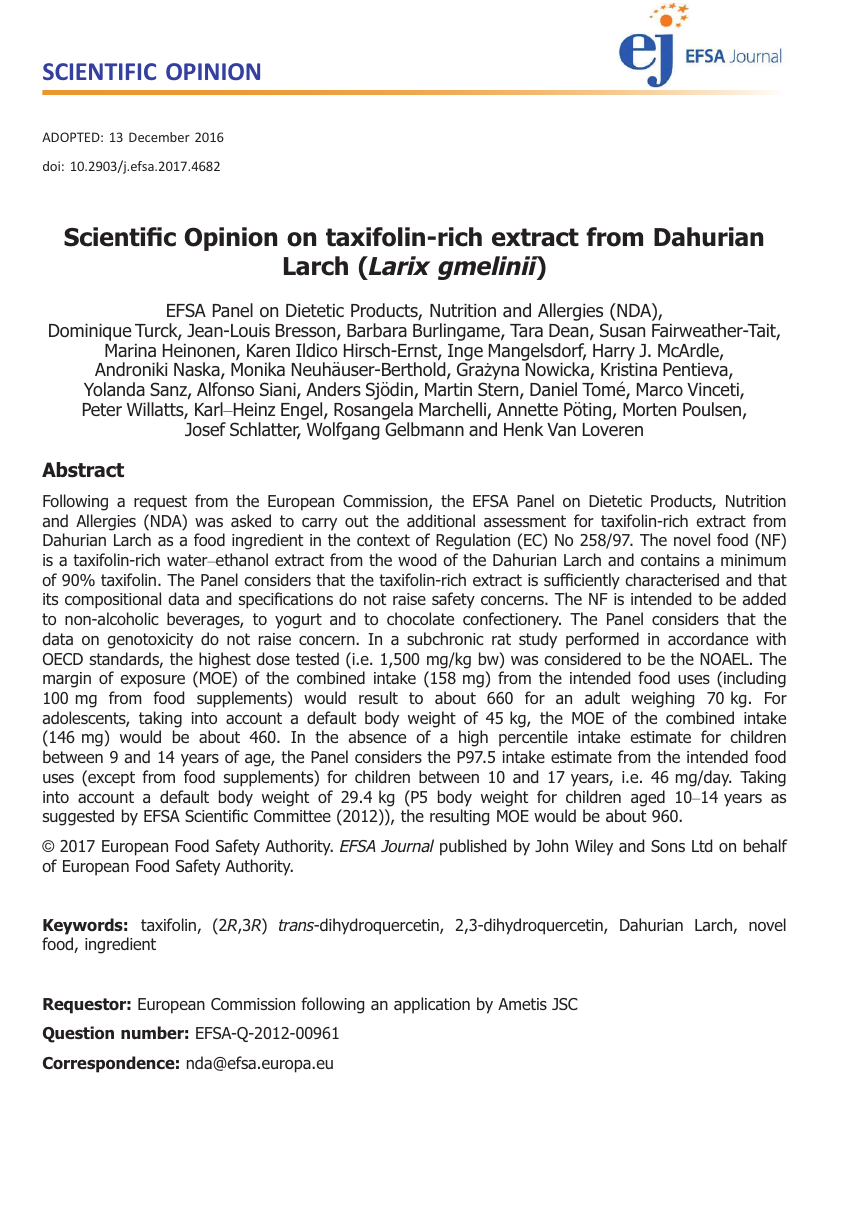
\includegraphics[width=0.3\textwidth]{group_A_1.png}}
\fbox{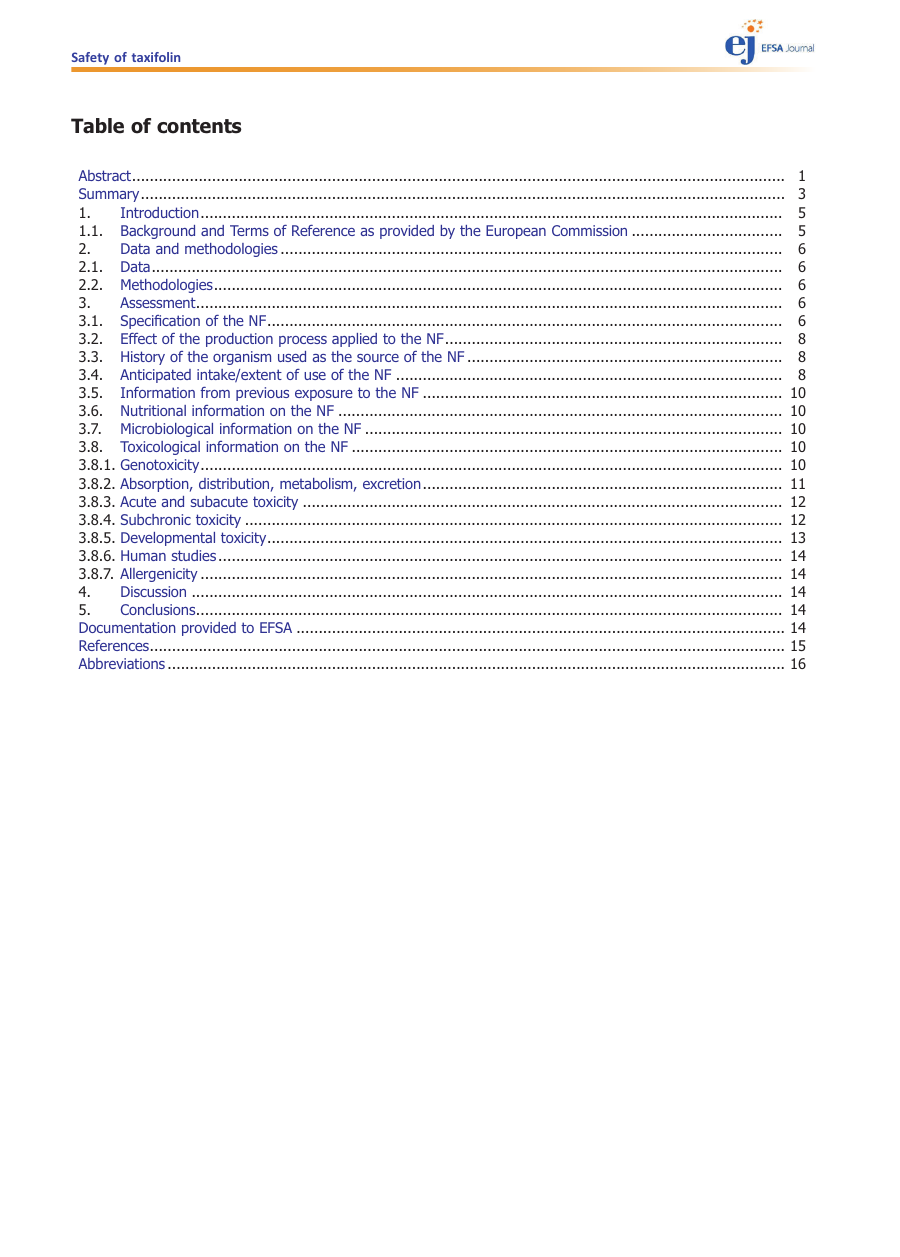
\includegraphics[width=0.3\textwidth]{group_A_2.png}}


\textbf{Group B}

This group has panel in the footnote and abstract on the first page.

\fbox{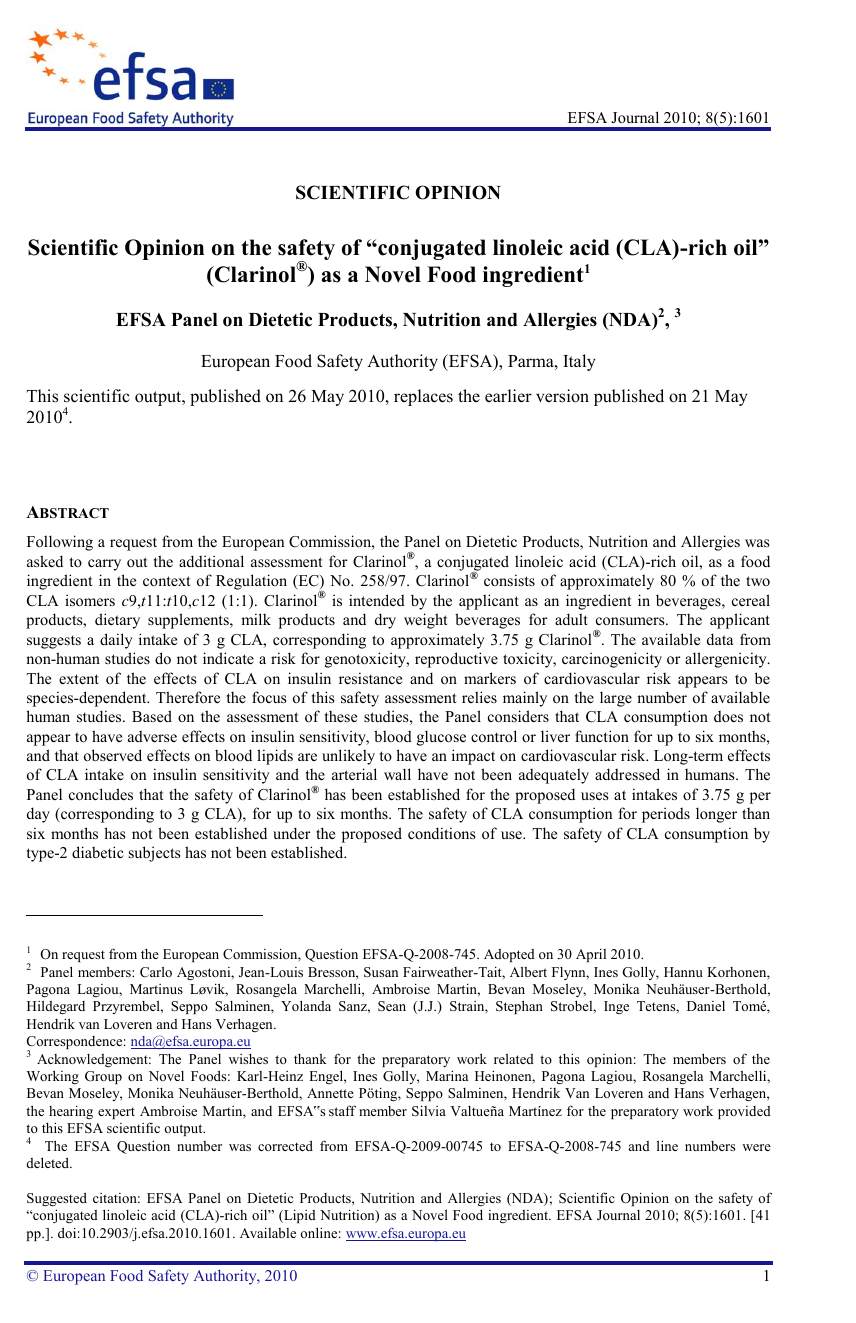
\includegraphics[width=0.3\textwidth]{group_B_1.png}}
\fbox{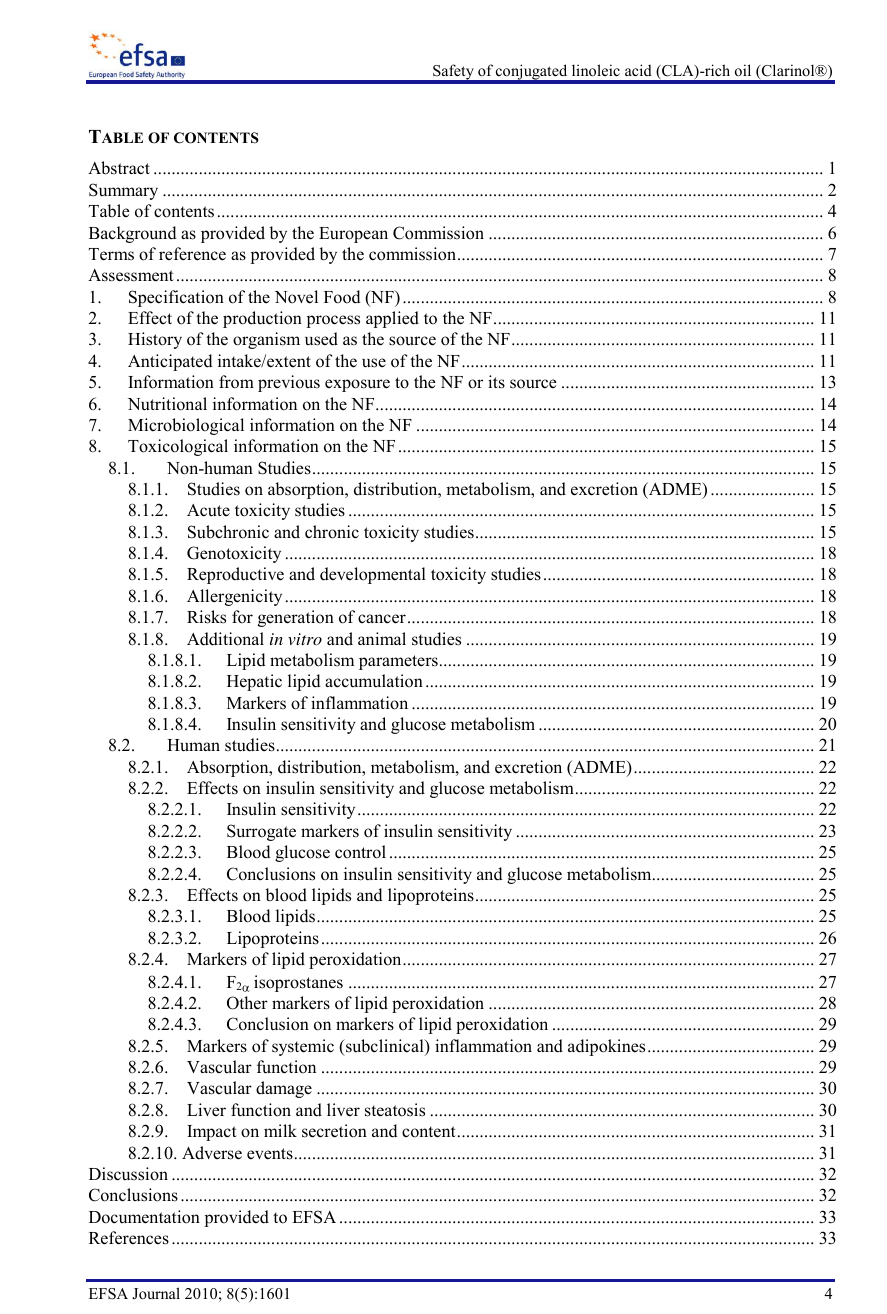
\includegraphics[width=0.3\textwidth]{group_B_2.png}}

\textbf{Group C}

This group has summary and keywords on the first page, and panel members on the last page.

\fbox{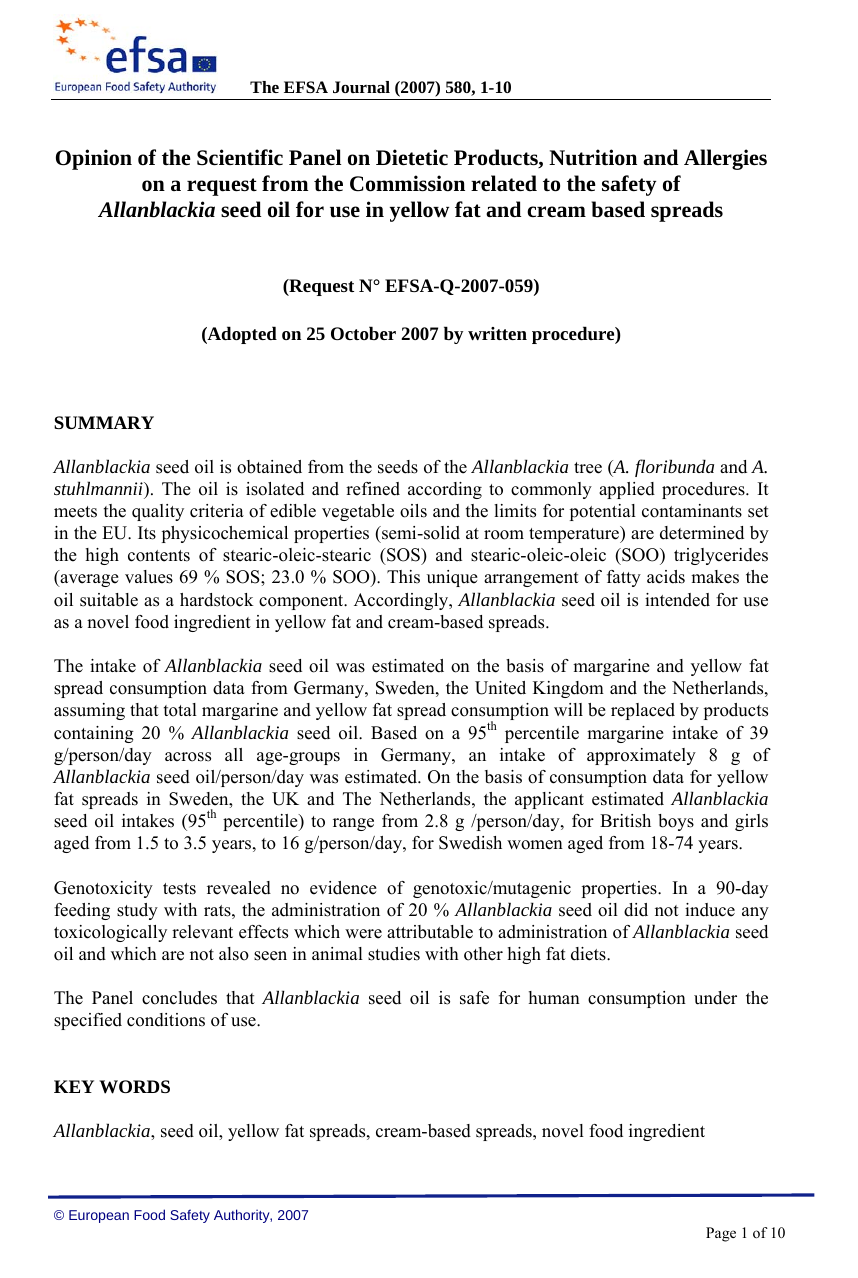
\includegraphics[width=0.3\textwidth]{group_C_1.png}}
\fbox{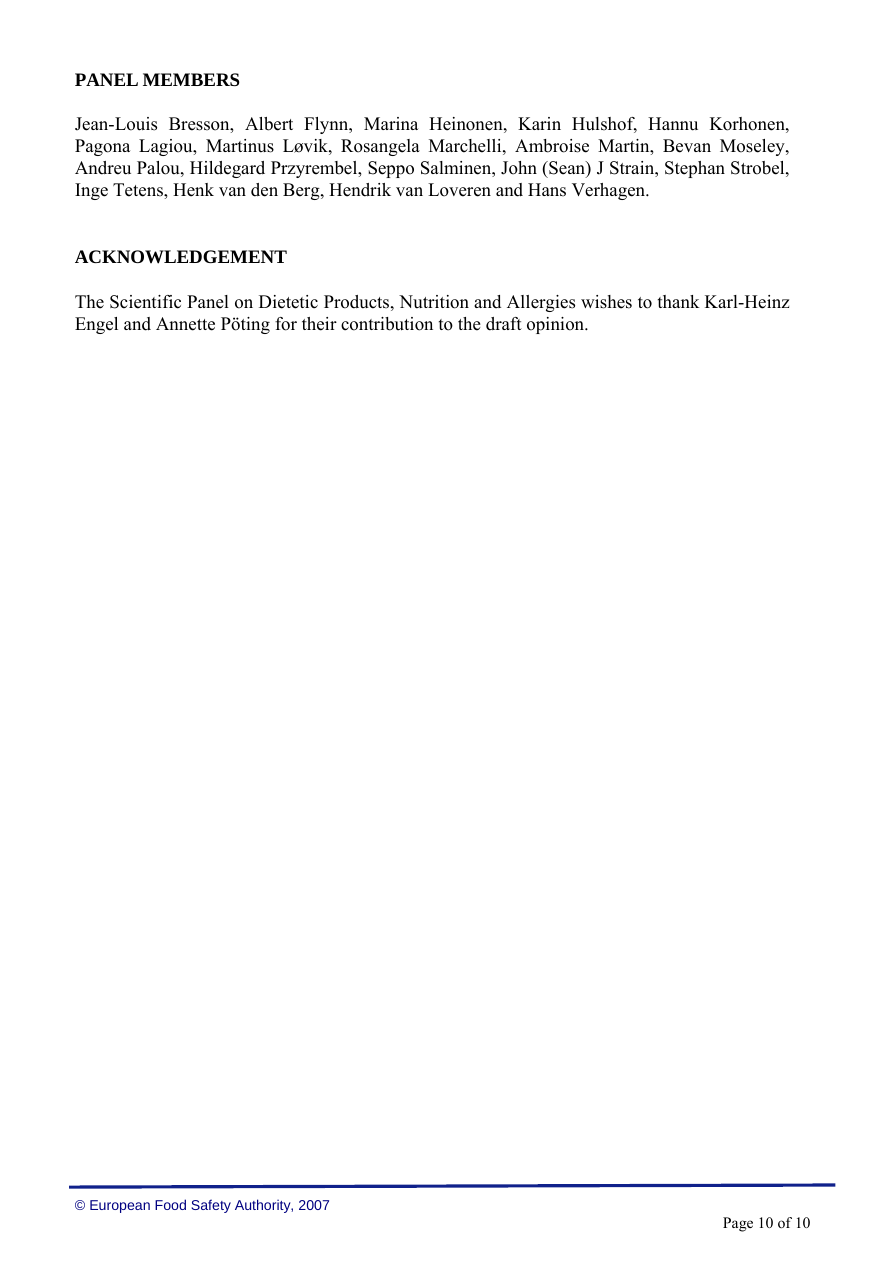
\includegraphics[width=0.3\textwidth]{group_C_2.png}}

\textbf{Group D}

This group has panel members on the first page, followed by summary and keywords.

\fbox{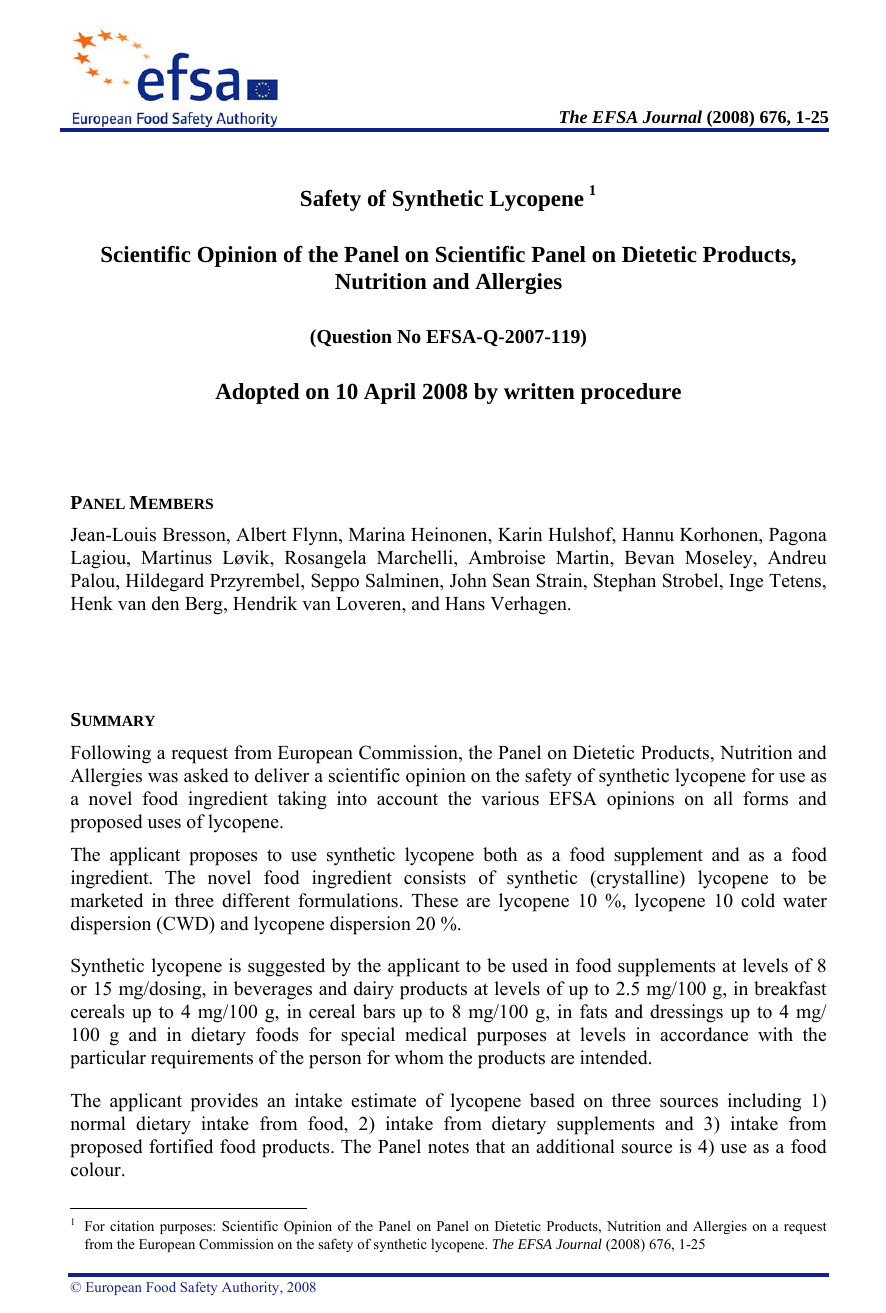
\includegraphics[width=0.3\textwidth]{group_D_1.png}}
\fbox{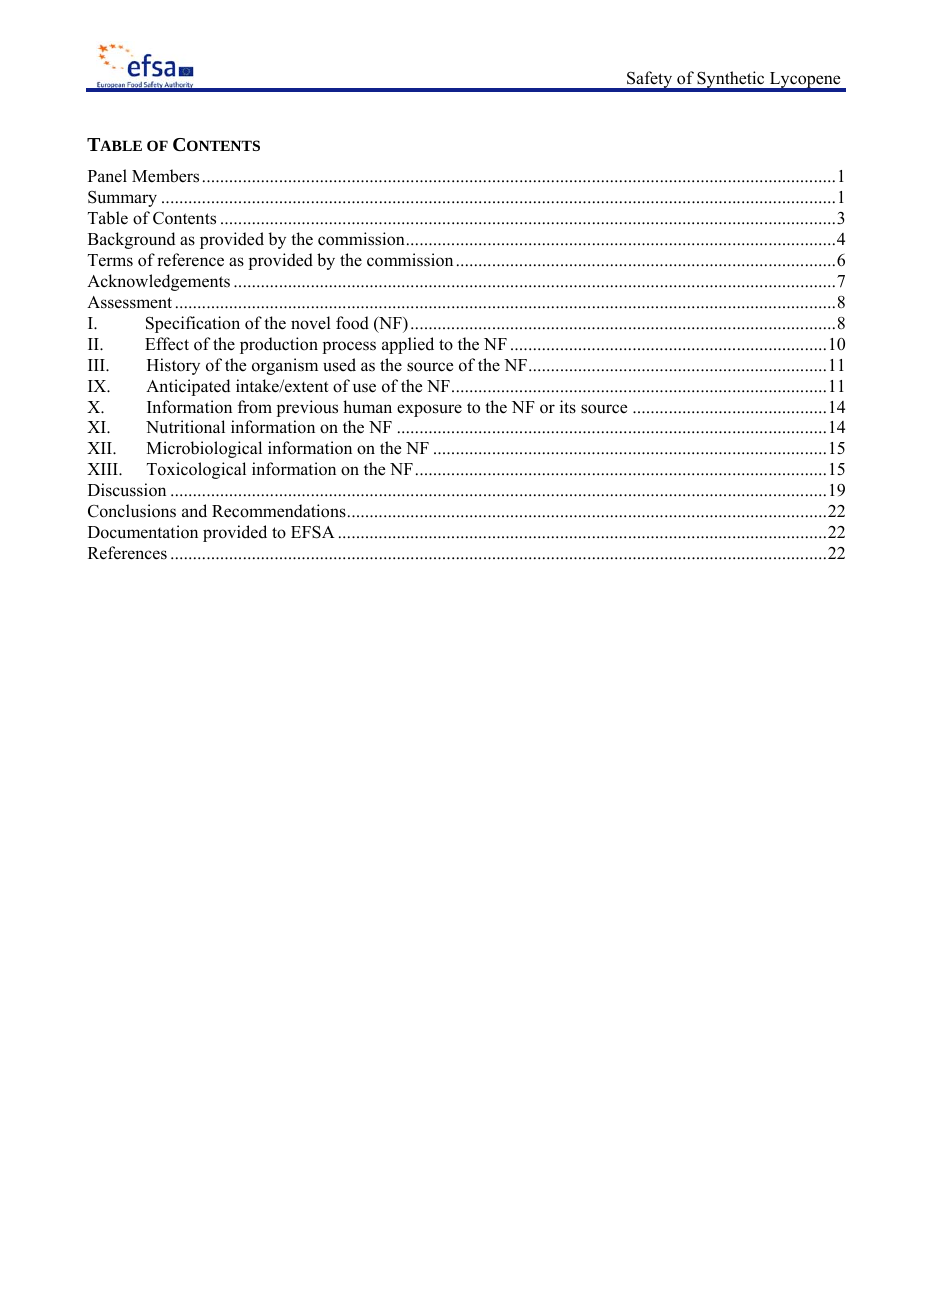
\includegraphics[width=0.3\textwidth]{group_D_2.png}}

\textbf{Group E}

\fbox{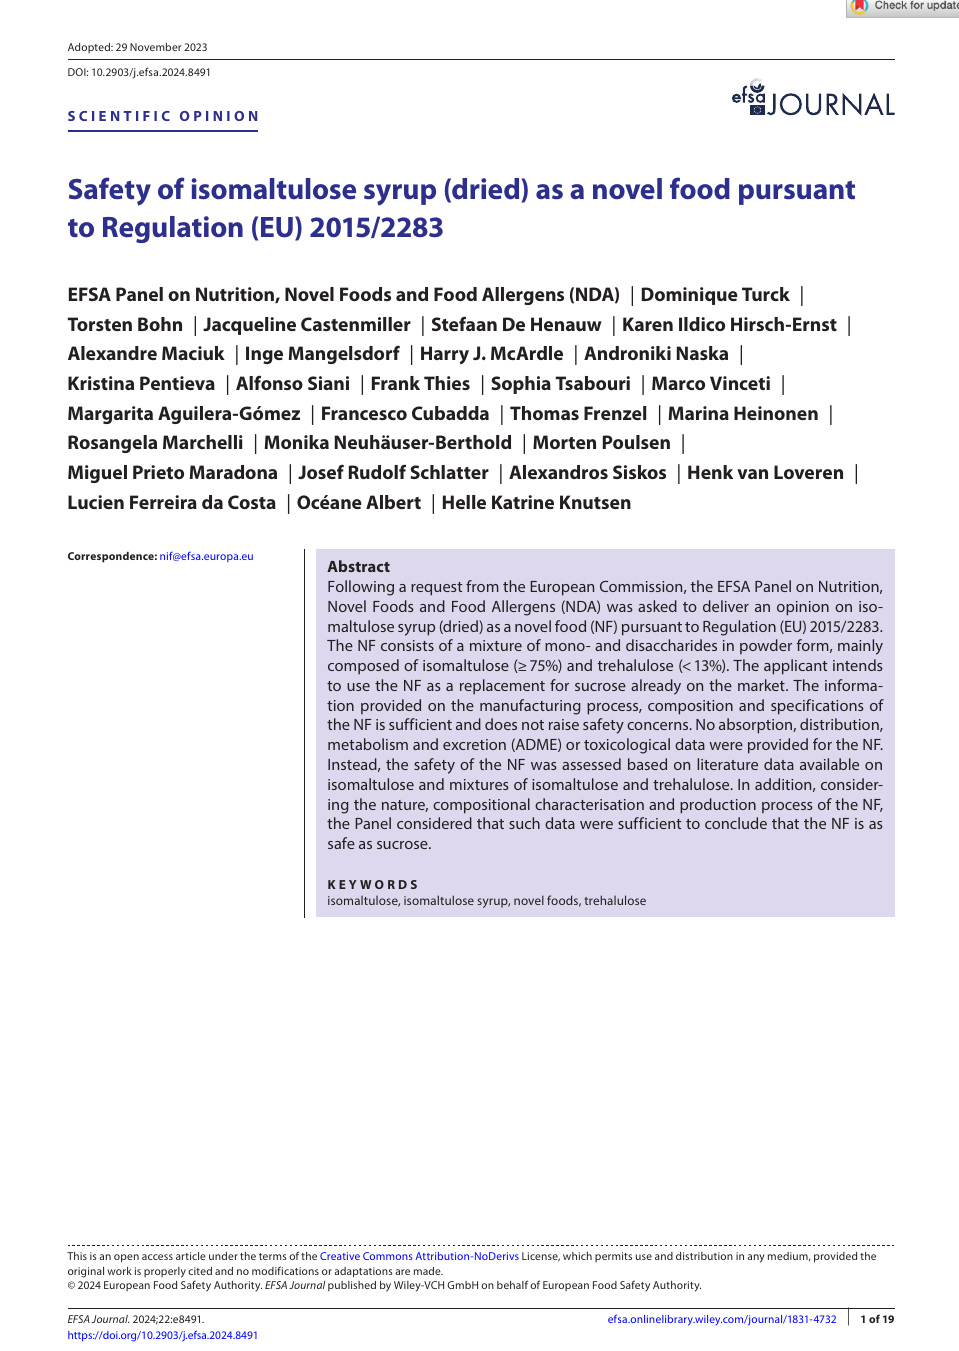
\includegraphics[width=0.3\textwidth]{group_E_1.png}}
\fbox{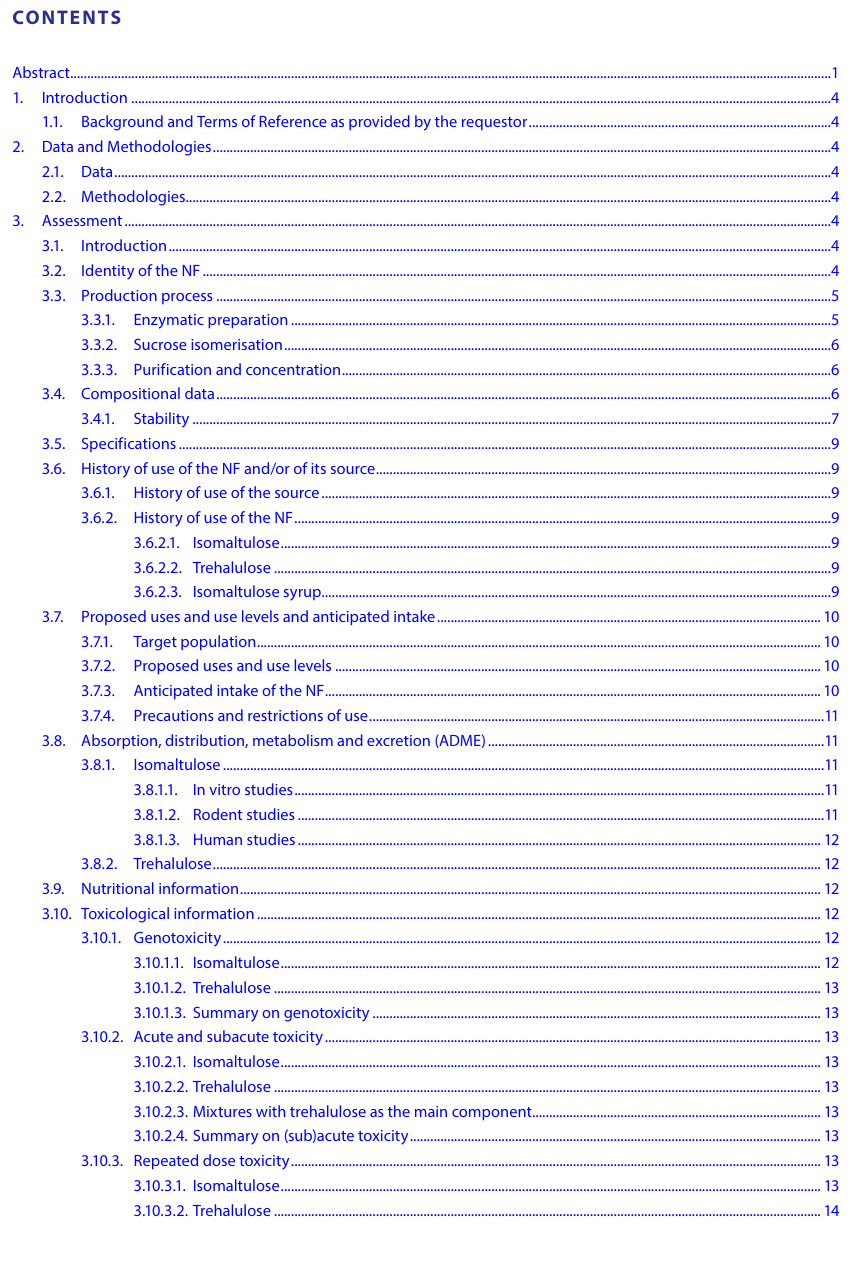
\includegraphics[width=0.3\textwidth]{group_E_2.png}}

The distribution in the groups is as follows:

\begin{center}
    \begin{tabular}{| l | l |}
    \hline
    \textbf{group} & \textbf{count} \\
    \hline
    A & 142 \\ 
    B & 32 \\  
    C & 4 \\
    D & 14 \\
    E & 6 \\
    \hline
    \end{tabular}
\end{center}

\section{Extraction rules}

- rozdelit na casti, ktere lze ziskat z FRONT

\subsection{DOI}
The DOI can be found in article-meta - article-id - pub-id-type="doi".

\lstset{language=XML, basicstyle=\footnotesize}
\begin{lstlisting}
<front>
    <article-meta>
        <article-id pub-id-type="doi">10.2903/j.efsa.2023.7904</article-id>
\end{lstlisting}

\subsection{Adoption date}
The traditional foods do not have adoption date, instead they have approval date, which is not included in the JATS files and therefore
cannot be extracted. The novel foods have adoption date.


front - notes -fn-group - v nejake z nich je Adopted
group6 - ADOPTED: in fn-group 
\lstset{language=XML, basicstyle=\footnotesize}
\begin{lstlisting}
<front>
    <notes>
        <fn-group>
            <fn id="efs26305-note-1203" xml:lang="en">
                <p>Adopted: 22 October 2020</p>
            </fn>
        </fn-group>
    </notes>
</front>
\end{lstlisting}

\subsection{Publication Date}
Publication date can be found in article-meta - pub-date - pub-type="epub".

\subsection{Question Number}

question number je taky v jedne fn-group

\lstset{language=XML}
\begin{lstlisting}
<front>
    <notes>
        <fn-group>
            <fn id="efs26305-note-1002" xml:lang="en">
                <p>
                    <bold>Question number:</bold>
                    EFSA-Q-2020-00491
                </p>
            </fn>
        </fn-group>
    </notes>
</front>
\end{lstlisting}

\subsection{Scientific Panels}
Usually NDA, for traditional foods EFSA, sometimes also GMO.


group 3 - v title: Panel on dietetic products, nutrition and allergies
group 6 - article-meta : contrib-group : collab(collab-type="authors") : NDA

look into collab - some panel there? (gmo, nda) -> added
                - no panel there?
                    - look into title ->some panel there -> added
                                        -> no panel there -> panel='EFSA'

ve formátu \textbf{Group 2} je to až někde úplně dole:
v body $\rightarrow$ pak najít sekci s tímto titlem

\lstset{language=XML}
\begin{lstlisting}
<sec id="efs28416-sec-0024" xml:lang="en">
    <title>QUESTION NUMBER</title>
    <p xml:lang="en">EFSA-Q-2020-00491</p>
</sec>
\end{lstlisting}

pro nalezeni pouzity regex: 
\lstset{language=Python}
\begin{lstlisting}
r'EFSA[-]Q[-]\S+'
\end{lstlisting}

\subsection{Scientific Officer}
EFSA provided us with list of possible scientific officers.
vic popsat jak toto funguje


\subsection{Mandate type}
--order matters

- guidance - always has guidance in the title
- traditional food - always have notification of XX as traditional food

- extension of use
- new dossier - the remaining ones


- nutrient source - can be added

\subsection{Novel Food Name}
- v title v article meta $\rightarrow$ article-title

\subsection{Category}
One NF can fall under multiple categories.
Categories as per Regulation Article 3 of 2015/2283.
Traditional food guidelines specify following categories

Categories are defined in specific european regulations. Each regulation defines its own set of categories.

REGULATION (EC) No 258 /97 from 27 January 1991

\begin{enumerate}[label=(\alph*)]
    \item foods and food ingredients containing or consisting of genetically modified organisms within the meaning of Directive 90 /220 /EEC;
    \item foods and food ingredients producted from, but not containing, genetically modified organisms;
    \item foods and food ingredients with a new or intentionally modified primary molecular structure;
    \item foods and food ingredients consisting of or isolated from micro-organisms, fungi or algae;
    \item foods and food ingredients consisting of or isolated from plants and food ingredients isolated from animals, except for foods and food ingredients obtained by traditional propagating or breeding prac­tices and having a history of safe food use;
    \item foods and food ingredients to which has been applied a production process not currently used, where that process gives rise to significant changes in the com­position or structure of the foods or food ingredients which affect their nutritional value, metabolism or level of undesirable substances .
\end{enumerate}

commission recommendation 97/618/EC from 29 July 1997

\begin{enumerate}[label=(\alph*)]
    \item pure chemicals or simple mixtures from non-GM sources;
    \item complex NF from non-GM source;
    \item GM plants and their products;
    \item GM animals and their products;
    \item GM microorganisms and their products;
    \item foods produced using a novel process.
\end{enumerate}

REGULATION (EU) 2015/2283 from 25 November 2015, Article 3

\begin{enumerate}[label=(\roman*)]
    \item food with a new or intentionally modified molecular structure, where that structure was not used as, or in, a food within the Union before 15 May 1997;
    \item food consisting of, isolated from or produced from microorganisms, fungi or algae;
    \item food consisting of, isolated from or produced from material of mineral origin;
    \item food consisting of, isolated from or produced from plants or their parts, except when the food has a history of safe food use within the Union and is consisting of, isolated from or produced from a plant or a variety of the same species obtained by:
    
    — traditional propagating practices which have been used for food production within the Union before
    15 May 1997; or

    — non-traditional propagating practices which have not been used for food production within the Union
    before 15 May 1997, where those practices do not give rise to significant changes in the composition or
    structure of the food affecting its nutritional value, metabolism or level of undesirable substances;
    \item food consisting of, isolated from or produced from animals or their parts, except for animals obtained by
    traditional breeding practices which have been used for food production within the Union before 15 May 1997
    and the food from those animals has a history of safe food use within the Union;
    \item food consisting of, isolated from or produced from cell culture or tissue culture derived from animals, plants,
    micro-organisms, fungi or algae;
    \item food resulting from a production process not used for food production within the Union before 15 May 1997,
    which gives rise to significant changes in the composition or structure of a food, affecting its nutritional value,
    metabolism or level of undesirable substances;
    \item  food consisting of engineered nanomaterials as defined in point (f) of this paragraph;
    \item  vitamins, minerals and other substances used in accordance with Directive 2002/46/EC, Regulation (EC)
    No 1925/2006 or Regulation (EU) No 609/2013, where:
    
    — a production process not used for food production within the Union before 15 May 1997 has been applied
    as referred to in point (a) (vii) of this paragraph; or
    
    — they contain or consist of engineered nanomaterials as defined in point (f) of this paragraph;
    \item food used exclusively in food supplements within the Union before 15 May 1997, where it is intended to be
    used in foods other than food supplements as defined in point (a) of Article 2 of Directive 2002/46/EC;
\end{enumerate}

\section{Composition extraction}
why was deemed important
how was performed - gpt assisstent + query
success rate

\section{Implementation}
-mozna neni potreba zas tak popisovat
Two main classes:

\textbf{JATS Opinion}
 
- encompass the formal parts of the opinion, abstract the inner structure of the opinions into common interface

- it will abstract the formal things about the article: DOI, Title, EFSA Question, adoption date, publication date,
URL, authors(panels)

- also it will abstract the different headings from different types of opinion and match them to the same structure

\textbf{Opinion} 

- the scientific opinion itself, it will accept JATS opinion in constructor

- it will have subclass for each category, which will contain the category specific information

- it will extract NF Name, Applicant, Country of origin, NF code, type of mandate, regulation, outcome,
common name, trade names, food form\\
- also proposed uses + target population\\
- availability of ADME studies\\
- allergenicity\\
- food category -- for FOODS\\
- for \textbf{Microorganisms}: type, genus, species, strain, QPS(?)\\
- for \textbf{Plants}: type, common name, botanical name, genus, species, part used\\
- for \textbf{Animals}: genus, species, subspecies, part used\\
- for \textbf{Cell or Tissue}: genus, species, cell type\\
- for \textbf{Chemicals}: common name, IUPAC name, CAS notation, SMILES, molecular formula, InChi


\end{document}
